\chapter{XÂY DỰNG VÀ ĐÁNH GIÁ MÔ HÌNH}
\label{chap:models}

Chương này trình bày bộ đặc trưng, lý do lựa chọn thuật toán, quy trình huấn luyện và kiểm định chéo, kết quả so sánh các mô hình với mô hình cơ sở, phân tích lỗi và các đặc trưng ảnh hưởng nhiều đến dự báo. Ở giai đoạn này, tập kiểm tra năm 2010 chưa được sử dụng; mọi kết quả là kết quả kiểm định chéo trên tập huấn luyện.

\section{Bộ đặc trưng}
\label{sec:features}

Với mỗi tầm dự báo $h$, bảng có giám sát gồm 21 đặc trưng chỉ dùng thông tin đến thời điểm gốc $t$ (Bảng~\ref{tab:features}). Các đặc trưng được chọn dựa trên kết quả khảo sát ở Chương~\ref{chap:data}.

\begin{table}[htbp]
    \centering
    \caption{Bộ đặc trưng dùng cho mô hình.}
    \label{tab:features}
    \small
    \begin{tabularx}{\textwidth}{|>{\raggedright\arraybackslash}p{2.6cm}|>{\raggedright\arraybackslash}p{5.6cm}|>{\raggedright\arraybackslash}X|}
        \hline
        \textbf{Nhóm} & \textbf{Đặc trưng} & \textbf{Căn cứ} \\ \hline
        Trễ (9) & $y_{t-k}$, $k \in \{0,1,2,3,5,11,23,47,167\}$ & Tự tương quan cao ở vài giờ gần nhất và ở 24, 168 giờ (Hình~\ref{fig:acf}) \\ \hline
        Cùng giờ của mục tiêu (2) & $y_{t+h-24}$ (cùng giờ ngày trước), $y_{t+h-168}$ (cùng giờ tuần trước) & Chu kỳ ngày và tuần; cũng là đầu vào của SNaive24, SNaive168 \\ \hline
        Cửa sổ trượt (6) & Trung bình và độ lệch chuẩn của 3, 24, 168 giờ gần nhất, kết thúc tại $t$ & Mức nền và độ biến động gần đây \\ \hline
        Lịch (4) & Giờ, thứ, tháng, cờ cuối tuần của thời điểm mục tiêu $t+h$ & Mùa vụ theo giờ, tuần, năm (Hình~\ref{fig:label}, \ref{fig:daily}) \\ \hline
    \end{tabularx}
\end{table}

Notebook kiểm tra trực tiếp rằng bộ đặc trưng không dùng thông tin tương lai: thay toàn bộ giá trị sau một mốc $T$ bằng một giá trị vô lý, các đặc trưng tại mọi thời điểm $t \le T$ không thay đổi.

\section{Lựa chọn thuật toán}
\label{sec:algorithms}

Nhóm dùng bốn mô hình cơ sở theo~\eqref{eq:baselines}: Mean (trung bình nhãn của phần huấn luyện), Naive, SNaive24 và SNaive168. Ba mô hình học máy được chọn theo định hướng của đề tài và đặc điểm dữ liệu (Bảng~\ref{tab:algorithms}).

\begin{table}[htbp]
    \centering
    \caption{Lý do lựa chọn và cấu hình các mô hình học máy.}
    \label{tab:algorithms}
    \small
    \begin{tabularx}{\textwidth}{|>{\raggedright\arraybackslash}p{2.5cm}|>{\raggedright\arraybackslash}X|>{\raggedright\arraybackslash}p{4.6cm}|}
        \hline
        \textbf{Mô hình} & \textbf{Lý do lựa chọn} & \textbf{Tiền xử lý và siêu tham số} \\ \hline
        Linear Regression & Mô hình tham số đơn giản nhất, dễ diễn giải; kiểm tra phần quan hệ tuyến tính giữa nhãn và các giá trị trễ. & One-hot giờ, thứ, tháng (bỏ một mức mỗi nhóm); điền trung vị và chuẩn hóa cột số. \\ \hline
        Random Forest & Học được quan hệ phi tuyến và tương tác giờ $\times$ thứ $\times$ tháng mà khảo sát đã chỉ ra; lấy trung bình nhiều cây giúp giảm phương sai. & Điền trung vị; 300 cây; tối thiểu 5 mẫu ở mỗi lá; mỗi lần tách xét 50\% số đặc trưng. \\ \hline
        XGBoost & Boosting cây thường cho sai số thấp trên dữ liệu dạng bảng khoảng vài chục nghìn mẫu; xử lý trực tiếp giá trị thiếu sau các khối dữ liệu thiếu. & 400 cây; tốc độ học 0,05; độ sâu tối đa 6; tổng trọng số tối thiểu ở lá 5; mỗi cây dùng 80\% số mẫu và 80\% số đặc trưng. \\ \hline
    \end{tabularx}
\end{table}

Siêu tham số được cố định trước ở các giá trị phổ biến và không được chọn theo kết quả kiểm định. Việc dò tìm siêu tham số trên kiểm định chéo thuộc giai đoạn tối ưu hóa ở bước tiếp theo; tách hai giai đoạn giúp đo được tác động của việc tối ưu. Mọi mô hình cố định hạt giống ngẫu nhiên bằng 42 để kết quả tái lập được.

\section{Quy trình huấn luyện và đánh giá}
\label{sec:protocol}

Mỗi mô hình học máy được tổ chức thành một Pipeline gồm các bước tiền xử lý và mô hình. Quy trình kiểm định chéo trên tập huấn luyện như sau:
\begin{enumerate}
    \item Dùng 5 fold TimeSeriesSplit như Bảng~\ref{tab:folds}; mỗi tầm dự báo $h$ huấn luyện một mô hình riêng.
    \item Ở mỗi fold, Pipeline được khớp lại chỉ trên phần huấn luyện của fold đó, nên giá trị điền khuyết và tham số chuẩn hóa không chứa thông tin của phần kiểm định.
    \item Mọi mô hình được chấm trên cùng tập mẫu kiểm định: bỏ các giờ mà mô hình cơ sở thiếu giá trị quá khứ (sau các khối dữ liệu thiếu). Mỗi fold còn 2.080--2.160 mẫu, tổng cộng khoảng 10.670 mẫu cho mỗi $h$.
    \item Ghi lại MAE, RMSE, MAPE trên phần kiểm định và trên phần huấn luyện (trong mẫu) để nhận diện quá khớp; báo cáo trung bình $\pm$ độ lệch chuẩn qua 5 fold.
\end{enumerate}
Toàn bộ quy trình chạy trong khoảng 2 phút trên máy 16 luồng. Chạy lại từ đầu trong một môi trường ảo mới (tự tải dữ liệu từ UCI) cho kết quả trùng khớp đến sai số làm tròn ($10^{-14}$).

\section{Kết quả kiểm định chéo}
\label{sec:cv_results}

\begin{table}[htbp]
\centering
\caption[Kết quả kiểm định chéo của mọi mô hình]{Kết quả kiểm định chéo 5 fold trên tập huấn luyện (trung bình $\pm$ độ lệch chuẩn qua các fold).}
\label{tab:cv_summary}
\small
\begin{tabular}{|c|l|c|c|c|}
\hline
\textbf{$h$} & \textbf{Mô hình} & \textbf{MAE (kWh)} & \textbf{RMSE (kWh)} & \textbf{MAPE (\%)} \\
\hline
\multirow{7}{*}{1} & Mean & 0{,}708 $\pm$ 0{,}068 & 0{,}867 $\pm$ 0{,}128 & 112{,}2 $\pm$ 28{,}3 \\
\cline{2-5}
 & Naive & 0{,}440 $\pm$ 0{,}069 & 0{,}667 $\pm$ 0{,}087 & 46{,}4 $\pm$ 1{,}9 \\
\cline{2-5}
 & SNaive24 & 0{,}630 $\pm$ 0{,}128 & 0{,}919 $\pm$ 0{,}169 & 76{,}7 $\pm$ 5{,}6 \\
\cline{2-5}
 & SNaive168 & 0{,}602 $\pm$ 0{,}127 & 0{,}883 $\pm$ 0{,}164 & 73{,}7 $\pm$ 11{,}4 \\
\cline{2-5}
 & LinearRegression & 0{,}384 $\pm$ 0{,}052 & 0{,}545 $\pm$ 0{,}073 & 48{,}3 $\pm$ 3{,}5 \\
\cline{2-5}
 & RandomForest & 0{,}365 $\pm$ 0{,}048 & 0{,}527 $\pm$ 0{,}074 & 44{,}4 $\pm$ 4{,}3 \\
\cline{2-5}
 & XGBoost & 0{,}366 $\pm$ 0{,}056 & 0{,}527 $\pm$ 0{,}078 & 44{,}3 $\pm$ 3{,}2 \\
\hline
\multirow{7}{*}{6} & Mean & 0{,}708 $\pm$ 0{,}068 & 0{,}867 $\pm$ 0{,}128 & 112{,}2 $\pm$ 28{,}4 \\
\cline{2-5}
 & Naive & 0{,}971 $\pm$ 0{,}186 & 1{,}242 $\pm$ 0{,}201 & 145{,}0 $\pm$ 14{,}9 \\
\cline{2-5}
 & SNaive24 & 0{,}629 $\pm$ 0{,}127 & 0{,}918 $\pm$ 0{,}168 & 76{,}6 $\pm$ 5{,}5 \\
\cline{2-5}
 & SNaive168 & 0{,}602 $\pm$ 0{,}127 & 0{,}883 $\pm$ 0{,}164 & 73{,}7 $\pm$ 11{,}4 \\
\cline{2-5}
 & LinearRegression & 0{,}508 $\pm$ 0{,}081 & 0{,}678 $\pm$ 0{,}110 & 73{,}6 $\pm$ 7{,}9 \\
\cline{2-5}
 & RandomForest & 0{,}482 $\pm$ 0{,}078 & 0{,}660 $\pm$ 0{,}114 & 66{,}6 $\pm$ 7{,}1 \\
\cline{2-5}
 & XGBoost & 0{,}488 $\pm$ 0{,}107 & 0{,}667 $\pm$ 0{,}138 & 66{,}8 $\pm$ 9{,}9 \\
\hline
\multirow{7}{*}{12} & Mean & 0{,}708 $\pm$ 0{,}068 & 0{,}867 $\pm$ 0{,}128 & 112{,}1 $\pm$ 28{,}5 \\
\cline{2-5}
 & Naive & 0{,}781 $\pm$ 0{,}207 & 1{,}068 $\pm$ 0{,}244 & 104{,}6 $\pm$ 23{,}1 \\
\cline{2-5}
 & SNaive24 & 0{,}630 $\pm$ 0{,}128 & 0{,}919 $\pm$ 0{,}169 & 76{,}7 $\pm$ 5{,}5 \\
\cline{2-5}
 & SNaive168 & 0{,}602 $\pm$ 0{,}127 & 0{,}882 $\pm$ 0{,}162 & 73{,}5 $\pm$ 10{,}9 \\
\cline{2-5}
 & LinearRegression & 0{,}509 $\pm$ 0{,}083 & 0{,}680 $\pm$ 0{,}112 & 73{,}5 $\pm$ 7{,}6 \\
\cline{2-5}
 & RandomForest & 0{,}488 $\pm$ 0{,}078 & 0{,}664 $\pm$ 0{,}117 & 68{,}3 $\pm$ 6{,}9 \\
\cline{2-5}
 & XGBoost & 0{,}488 $\pm$ 0{,}096 & 0{,}665 $\pm$ 0{,}127 & 67{,}5 $\pm$ 7{,}5 \\
\hline
\multirow{7}{*}{24} & Mean & 0{,}708 $\pm$ 0{,}068 & 0{,}868 $\pm$ 0{,}128 & 112{,}0 $\pm$ 28{,}3 \\
\cline{2-5}
 & Naive & 0{,}630 $\pm$ 0{,}128 & 0{,}920 $\pm$ 0{,}168 & 76{,}7 $\pm$ 5{,}6 \\
\cline{2-5}
 & SNaive24 & 0{,}630 $\pm$ 0{,}128 & 0{,}920 $\pm$ 0{,}168 & 76{,}7 $\pm$ 5{,}6 \\
\cline{2-5}
 & SNaive168 & 0{,}603 $\pm$ 0{,}127 & 0{,}884 $\pm$ 0{,}162 & 73{,}7 $\pm$ 11{,}4 \\
\cline{2-5}
 & LinearRegression & 0{,}507 $\pm$ 0{,}088 & 0{,}681 $\pm$ 0{,}117 & 73{,}1 $\pm$ 8{,}8 \\
\cline{2-5}
 & RandomForest & 0{,}495 $\pm$ 0{,}080 & 0{,}671 $\pm$ 0{,}120 & 70{,}1 $\pm$ 9{,}2 \\
\cline{2-5}
 & XGBoost & 0{,}507 $\pm$ 0{,}115 & 0{,}686 $\pm$ 0{,}153 & 72{,}1 $\pm$ 12{,}0 \\
\hline
\end{tabular}
\end{table}


\begin{figure}[htbp]
    \centering
    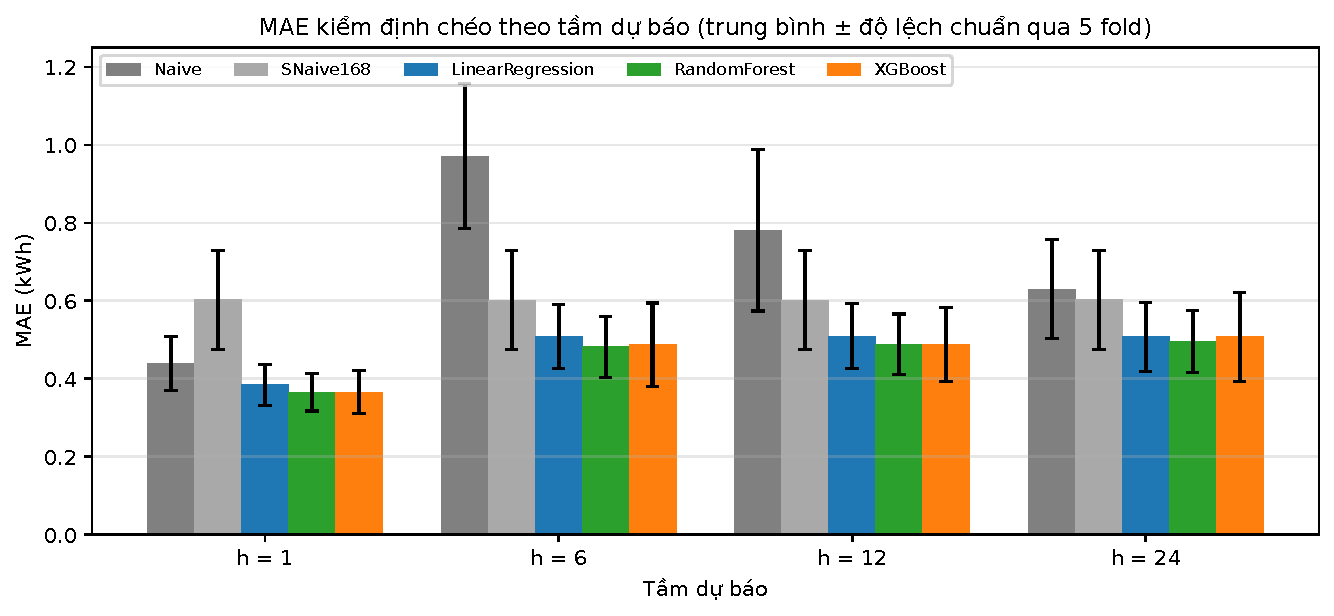
\includegraphics[width=0.92\textwidth]{figures/mae_theo_h.pdf}
    \caption{MAE kiểm định chéo theo tầm dự báo (trung bình $\pm$ độ lệch chuẩn qua 5 fold).}
    \label{fig:mae_h}
\end{figure}

\begin{table}[htbp]
\centering
\caption[So sánh mô hình học máy với mô hình cơ sở tốt nhất]{So sánh MAE trung bình của mô hình học máy với mô hình cơ sở tốt nhất ở từng tầm dự báo; cột cuối là số fold mô hình học máy có MAE thấp hơn.}
\label{tab:vs_baseline}
\small
\begin{tabular}{|c|c|l|c|c|c|}
\hline
\textbf{$h$} & \textbf{Cơ sở tốt nhất (MAE)} & \textbf{Mô hình} & \textbf{MAE} & \textbf{Giảm MAE (\%)} & \textbf{Số fold tốt hơn} \\
\hline
\multirow{3}{*}{1} & \multirow{3}{*}{Naive (0{,}440)} & LinearRegression & 0{,}384 & 12{,}7 & 5/5 \\
\cline{3-6}
 &  & RandomForest & 0{,}365 & 17{,}0 & 5/5 \\
\cline{3-6}
 &  & XGBoost & 0{,}366 & 16{,}9 & 5/5 \\
\hline
\multirow{3}{*}{6} & \multirow{3}{*}{SNaive168 (0{,}602)} & LinearRegression & 0{,}508 & 15{,}5 & 5/5 \\
\cline{3-6}
 &  & RandomForest & 0{,}482 & 20{,}0 & 5/5 \\
\cline{3-6}
 &  & XGBoost & 0{,}488 & 19{,}0 & 5/5 \\
\hline
\multirow{3}{*}{12} & \multirow{3}{*}{SNaive168 (0{,}602)} & LinearRegression & 0{,}509 & 15{,}4 & 5/5 \\
\cline{3-6}
 &  & RandomForest & 0{,}488 & 18{,}9 & 5/5 \\
\cline{3-6}
 &  & XGBoost & 0{,}488 & 18{,}8 & 5/5 \\
\hline
\multirow{3}{*}{24} & \multirow{3}{*}{SNaive168 (0{,}603)} & LinearRegression & 0{,}507 & 15{,}8 & 5/5 \\
\cline{3-6}
 &  & RandomForest & 0{,}495 & 17{,}8 & 5/5 \\
\cline{3-6}
 &  & XGBoost & 0{,}507 & 15{,}8 & 5/5 \\
\hline
\end{tabular}
\end{table}


Từ Bảng~\ref{tab:cv_summary}, Bảng~\ref{tab:vs_baseline} và Hình~\ref{fig:mae_h}:
\begin{enumerate}
    \item Cả ba mô hình học máy vượt mọi mô hình cơ sở ở mọi tầm dự báo và ở cả 5/5 fold, giảm MAE 12,7--20,0\% so với mô hình cơ sở tốt nhất. Mức mong muốn giảm ít nhất 10\% đặt ra ở Bảng~\ref{tab:objectives} đạt được với cả ba mô hình.
    \item Mô hình cơ sở tốt nhất thay đổi theo $h$. Naive tốt nhất ở $h = 1$ (MAE 0,440 kWh) nhưng kém nhất ở $h = 6$ (0,971 kWh, kém cả Mean), đúng như tự tương quan gần bằng 0 ở độ trễ 6. Từ $h = 6$, SNaive168 tốt nhất (khoảng 0,602 kWh).
    \item Random Forest có MAE thấp nhất hoặc ngang thấp nhất ở cả bốn tầm dự báo: 0,365 kWh ở $h = 1$ và 0,482--0,495 kWh ở $h \ge 6$. XGBoost gần như ngang Random Forest ở $h \le 12$ (chênh lệch không quá 0,006 kWh), nhưng ở $h = 24$ chỉ ngang Linear Regression (0,507 kWh) và có độ lệch chuẩn giữa các fold lớn nhất (0,115). Linear Regression kém hai mô hình cây 0,01--0,03 kWh.
    \item Các chênh lệch giữa ba mô hình học máy nhỏ hơn độ lệch chuẩn giữa các fold (0,05--0,12 kWh), nên với 5 fold chưa thể kết luận chắc chắn mô hình nào tốt nhất; chênh lệch giữa mô hình học máy và mô hình cơ sở thì rõ ràng và nhất quán ở mọi fold.
    \item MAPE của mô hình học máy vẫn cao (44--73\%) dù MAE dưới 0,51 kWh, do nhiều giờ có điện năng rất nhỏ. Điều này khớp với lý do không dùng MAPE làm chỉ số chính.
\end{enumerate}

\begin{figure}[htbp]
    \centering
    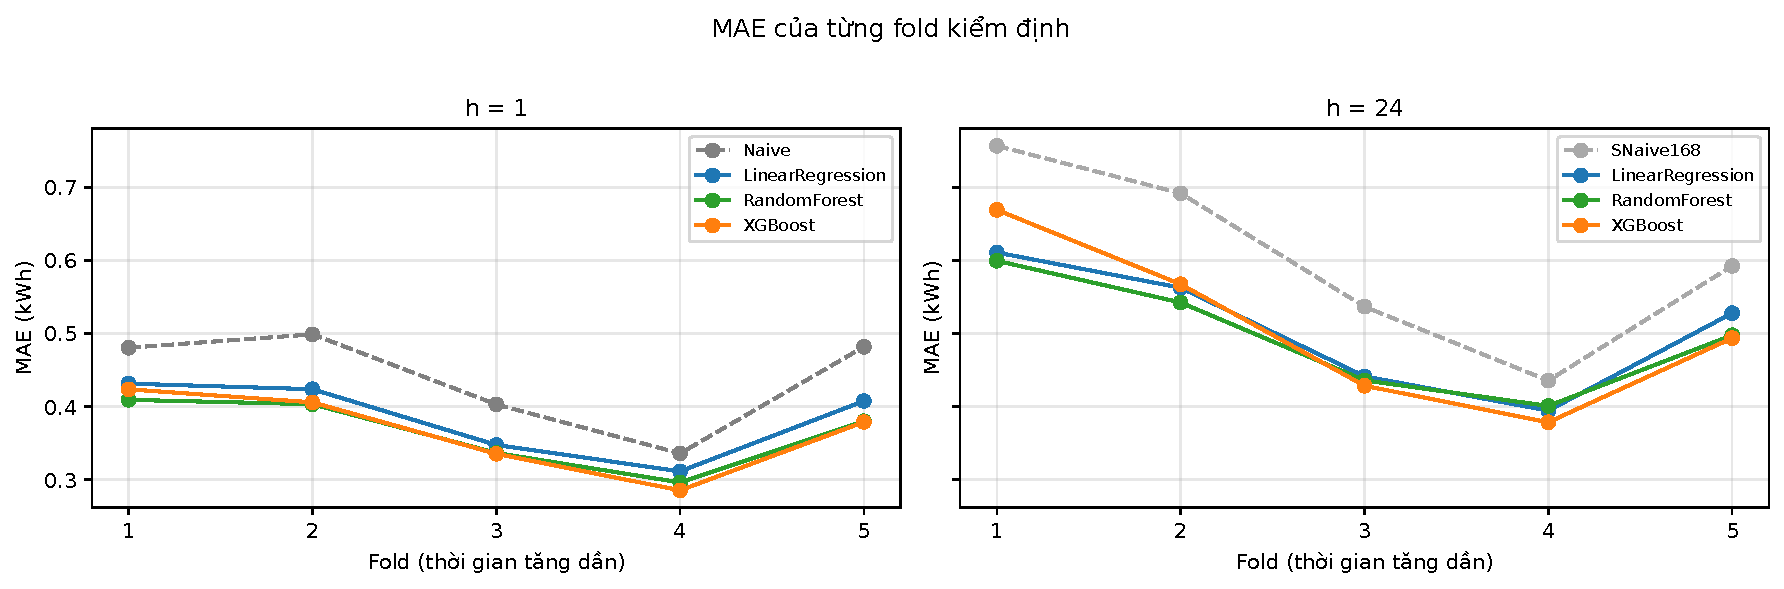
\includegraphics[width=\textwidth]{figures/mae_theo_fold.pdf}
    \caption{MAE của từng fold kiểm định với $h = 1$ (trái) và $h = 24$ (phải).}
    \label{fig:mae_fold}
\end{figure}

Hình~\ref{fig:mae_fold} cho thấy thứ hạng các mô hình gần như giữ nguyên qua các fold, còn mức sai số thay đổi theo mùa của phần kiểm định: fold 4 (07--10/2009, có tháng 8 tiêu thụ thấp) có MAE thấp nhất, fold 1 và 2 (mùa đông) cao nhất. Độ lệch chuẩn giữa các fold vì vậy chủ yếu phản ánh mức tiêu thụ của từng giai đoạn.

\section{Sai số trên phần huấn luyện và phần kiểm định}
\label{sec:train_val}

\begin{table}[htbp]
\centering
\caption[MAE trên phần huấn luyện và phần kiểm định]{MAE trung bình qua 5 fold trên phần huấn luyện (trong mẫu, ký hiệu HL) và phần kiểm định (KĐ), cùng tỷ số KĐ/HL.}
\label{tab:train_val}
\small
\begin{tabular}{|c|c|c|c|c|c|c|c|c|c|}
\hline
\multirow{2}{*}{\textbf{$h$}} & \multicolumn{3}{c|}{\textbf{Linear Regression}} & \multicolumn{3}{c|}{\textbf{Random Forest}} & \multicolumn{3}{c|}{\textbf{XGBoost}} \\
\cline{2-10}
 & HL & KĐ & KĐ/HL & HL & KĐ & KĐ/HL & HL & KĐ & KĐ/HL \\
\hline
1 & 0{,}409 & 0{,}384 & 0{,}94 & 0{,}241 & 0{,}365 & 1{,}51 & 0{,}265 & 0{,}366 & 1{,}38 \\ \hline
6 & 0{,}551 & 0{,}508 & 0{,}92 & 0{,}304 & 0{,}482 & 1{,}58 & 0{,}334 & 0{,}488 & 1{,}46 \\ \hline
12 & 0{,}551 & 0{,}509 & 0{,}93 & 0{,}308 & 0{,}488 & 1{,}59 & 0{,}338 & 0{,}488 & 1{,}45 \\ \hline
24 & 0{,}549 & 0{,}507 & 0{,}92 & 0{,}311 & 0{,}495 & 1{,}59 & 0{,}339 & 0{,}507 & 1{,}50 \\ \hline
\end{tabular}
\end{table}


\begin{figure}[htbp]
    \centering
    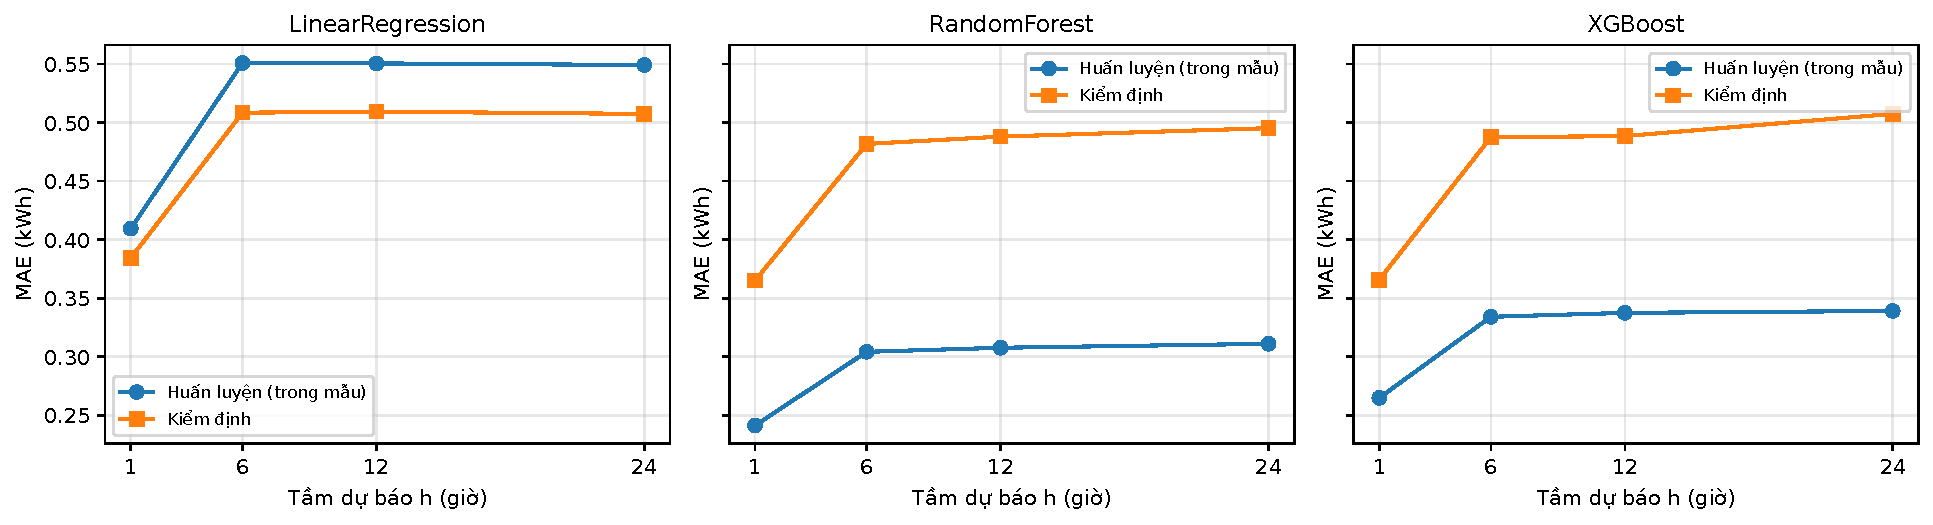
\includegraphics[width=\textwidth]{figures/train_val.pdf}
    \caption{MAE trên phần huấn luyện (trong mẫu) và phần kiểm định theo tầm dự báo.}
    \label{fig:train_val}
\end{figure}

Bảng~\ref{tab:train_val} và Hình~\ref{fig:train_val} cho thấy hai hành vi khác nhau:
\begin{itemize}
    \item Random Forest và XGBoost có MAE huấn luyện chỉ 0,24--0,34 kWh trong khi MAE kiểm định là 0,37--0,51 kWh (gấp 1,4--1,6 lần), và khoảng cách này xuất hiện ở mọi fold. Đây là dấu hiệu quá khớp. Tuy nhiên sai số huấn luyện ở đây là sai số trong mẫu, vốn luôn thấp với mô hình cây (mỗi lá của Random Forest chỉ cần 5 mẫu), nên cần kiểm chứng thêm bằng đường cong học tập và đường cong kiểm định ở giai đoạn tối ưu hóa.
    \item Linear Regression có sai số huấn luyện (0,41--0,55 kWh) xấp xỉ sai số kiểm định và cao hơn hẳn sai số huấn luyện của mô hình cây, tức mô hình chưa khớp: quan hệ tuyến tính không biểu diễn được tương tác giữa lịch và mức tiêu thụ gần đây. Sai số huấn luyện còn hơi lớn hơn sai số kiểm định vì phần huấn luyện chứa các mùa đông 2006--2008 tiêu thụ cao.
\end{itemize}

\section{Phân tích lỗi}
\label{sec:error_analysis}

Phân tích dùng dự báo của mọi mô hình trên phần kiểm định của cả 5 fold (từ 10/2008 đến 12/2009). Các hình dưới đây trình bày $h = 1$ và $h = 24$, hai đầu của dải tầm dự báo.

\begin{figure}[htbp]
    \centering
    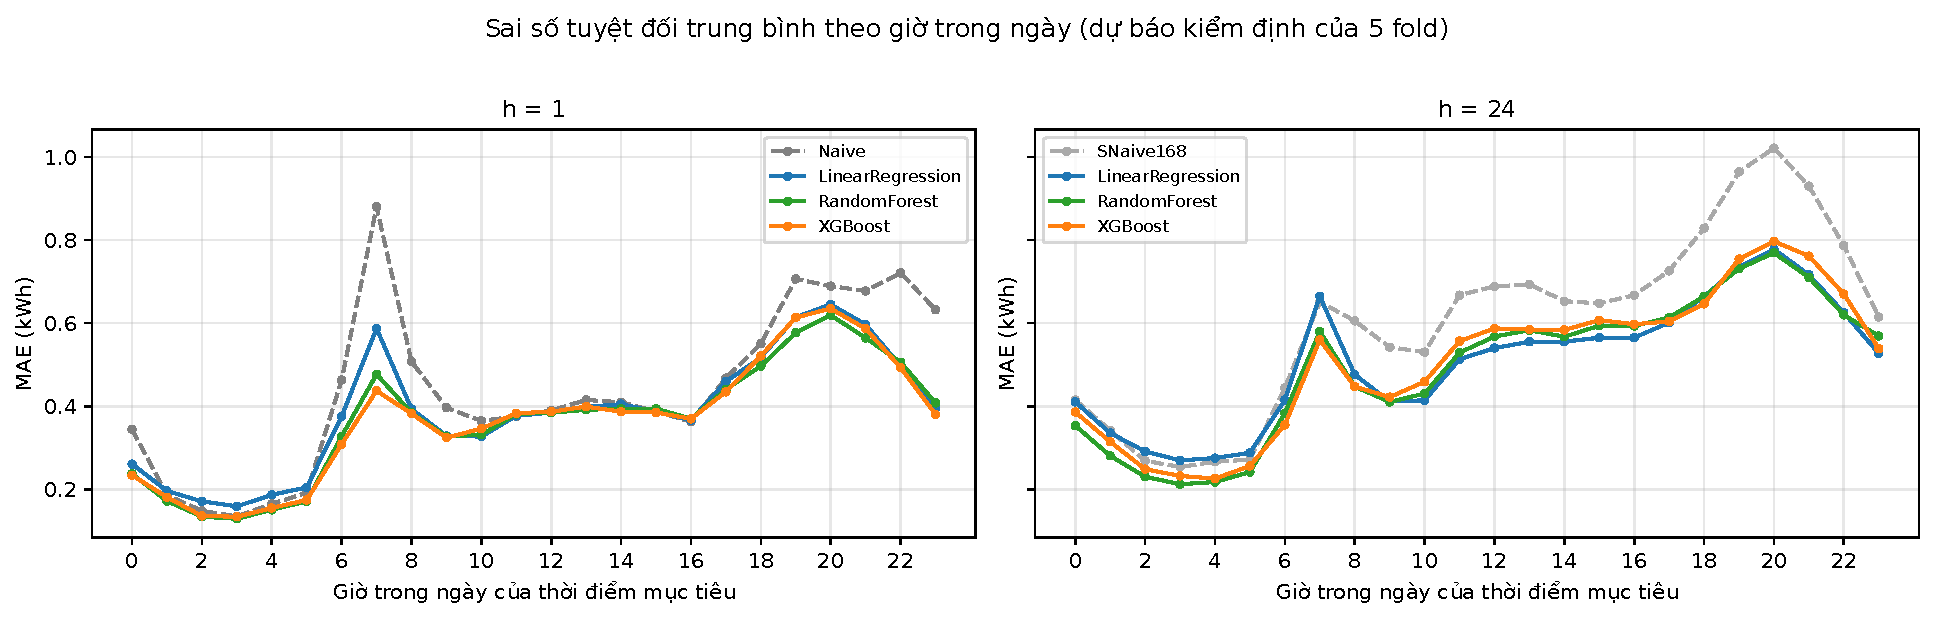
\includegraphics[width=\textwidth]{figures/mae_theo_gio.pdf}
    \caption{MAE theo giờ trong ngày của thời điểm mục tiêu.}
    \label{fig:mae_hour}
\end{figure}

\paragraph{Theo giờ trong ngày (Hình~\ref{fig:mae_hour}).} Sai số nhỏ nhất vào ban đêm (3 giờ: 0,13--0,16 kWh ở $h = 1$), khi hộ chỉ dùng tải nền. Đỉnh buổi tối 19--21 giờ là vùng khó nhất ở cả hai tầm dự báo: MAE của mô hình học máy là 0,56--0,65 kWh ở $h = 1$ và 0,71--0,80 kWh ở $h = 24$. Mô hình học máy cải thiện mạnh nhất ở đỉnh buổi sáng 7 giờ với $h = 1$ (Naive 0,88 kWh; Random Forest 0,48; XGBoost 0,44): Naive lặp lại giá trị 6 giờ còn thấp nên luôn trễ một bước khi tiêu thụ tăng, còn mô hình học máy biết từ đặc trưng giờ rằng 7 giờ thường tăng.

\begin{figure}[htbp]
    \centering
    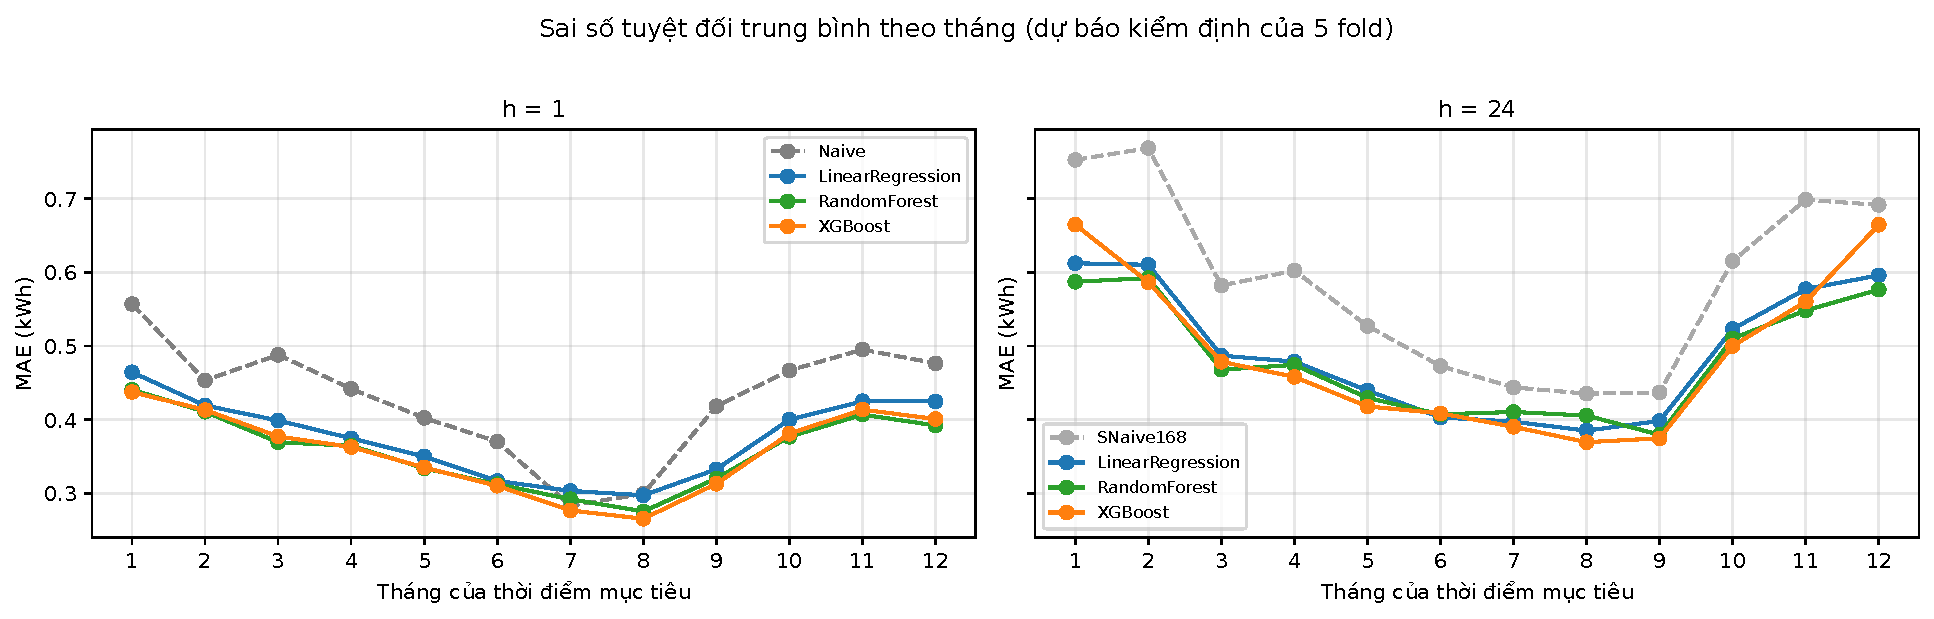
\includegraphics[width=\textwidth]{figures/mae_theo_thang.pdf}
    \caption{MAE theo tháng của thời điểm mục tiêu.}
    \label{fig:mae_month}
\end{figure}

\paragraph{Theo tháng (Hình~\ref{fig:mae_month}).} Sai số đi theo mức tiêu thụ: cao nhất vào mùa đông, thấp nhất vào tháng 7--8. Ở $h = 1$, tháng 7 là tháng duy nhất mô hình học máy không tốt hơn Naive rõ rệt (Naive 0,283; XGBoost 0,277; Linear Regression 0,303 kWh), vì khi tiêu thụ thấp và đều, giá trị giờ vừa qua đã là dự báo tốt. Ở $h = 24$, XGBoost có MAE tháng 1 và tháng 12 (cùng 0,665 kWh) cao hơn hẳn Random Forest (0,587 và 0,577), góp phần làm độ lệch chuẩn giữa các fold của XGBoost lớn hơn.

\begin{figure}[htbp]
    \centering
    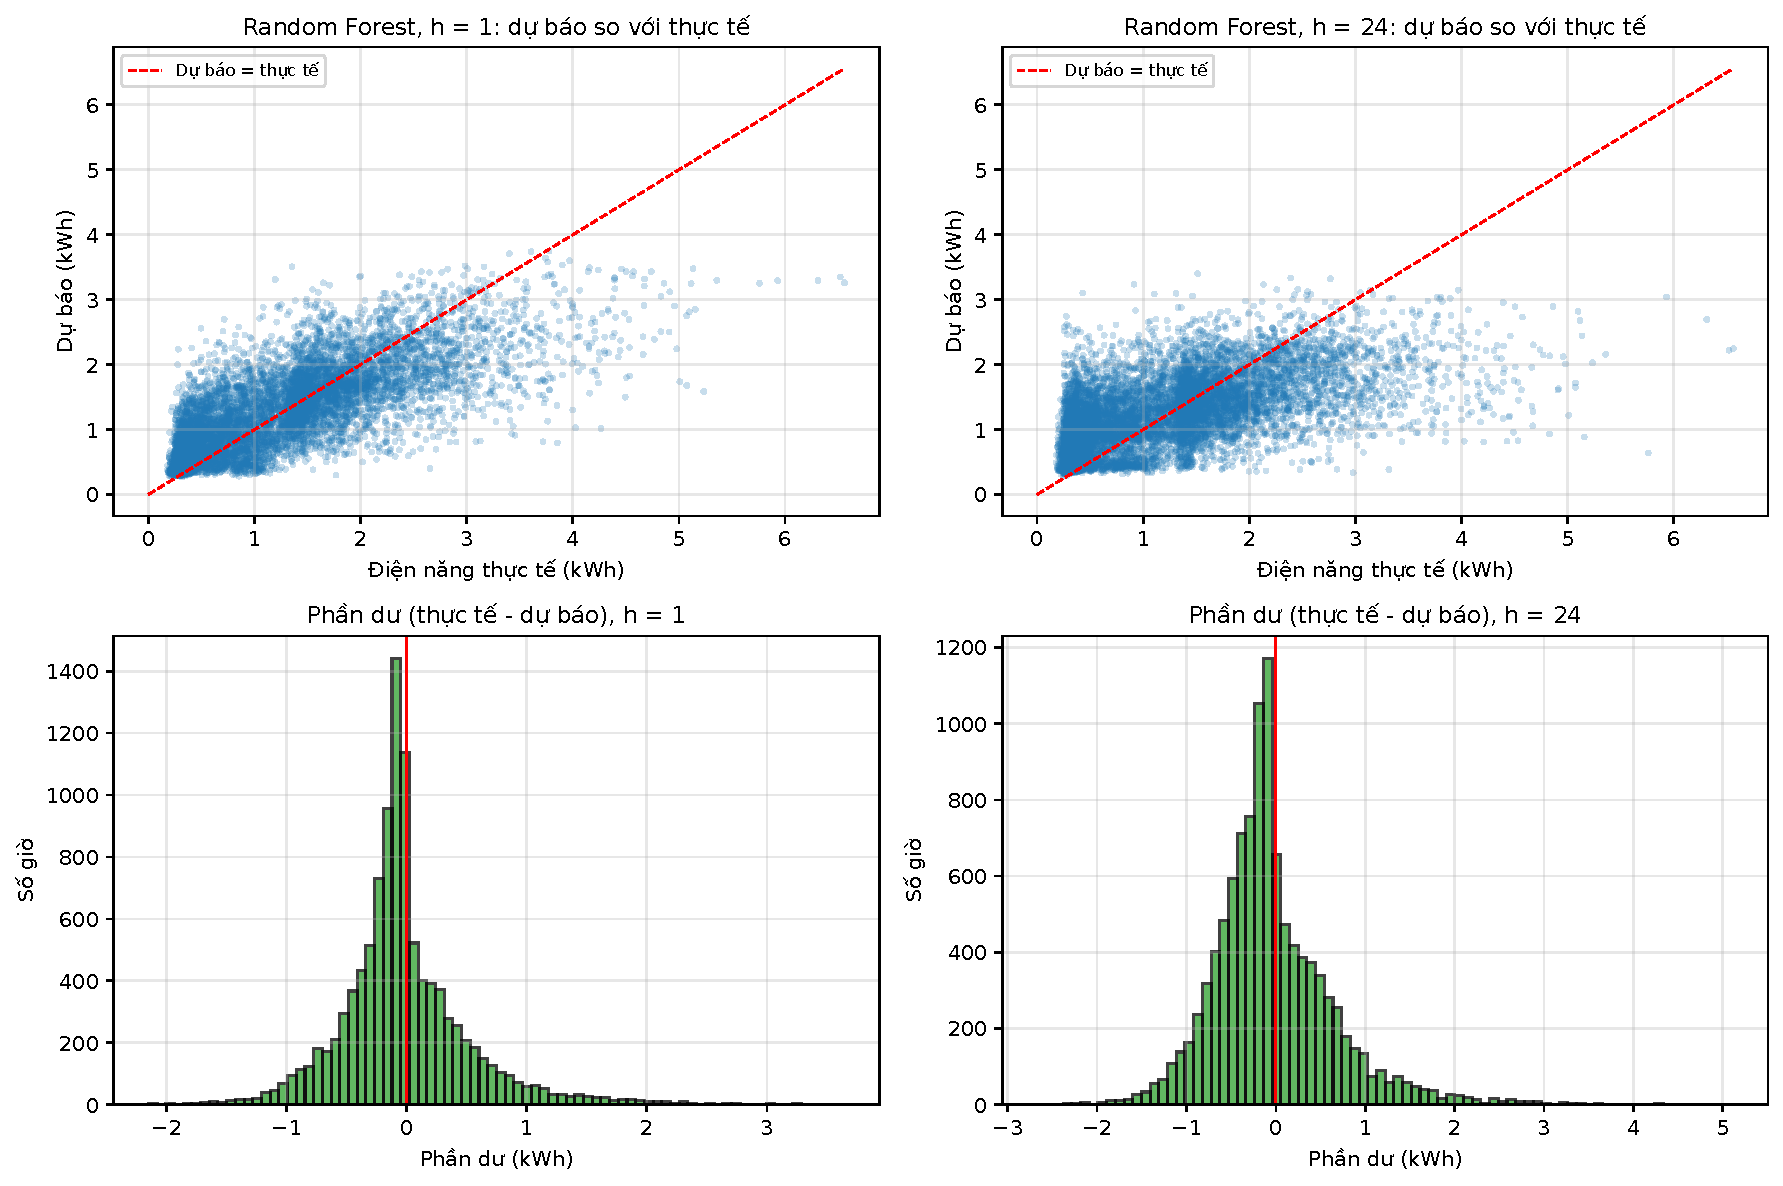
\includegraphics[width=0.95\textwidth]{figures/phan_du.pdf}
    \caption{Random Forest: dự báo so với thực tế (trên) và phân bố phần dư (dưới) với $h = 1$ và $h = 24$.}
    \label{fig:residuals}
\end{figure}

\begin{table}[htbp]
\centering
\caption[Mức độ tập trung của sai số]{Sai lệch trung bình (dự báo $-$ thực tế) ở nhóm giờ tiêu thụ cao nhất và thấp nhất, và tỷ trọng tổng sai số tuyệt đối do 10\% số giờ có sai số lớn nhất gây ra (dự báo kiểm định của 5 fold).}
\label{tab:error_conc}
\small
\begin{tabular}{|c|l|c|c|c|}
\hline
\textbf{$h$} & \textbf{Mô hình} & \textbf{5\% giờ cao nhất} & \textbf{10\% giờ thấp nhất} & \textbf{Tỷ trọng (\%)} \\
\hline
1 & LinearRegression & $-$1{,}112 & 0{,}214 & 33{,}2 \\ \hline
1 & RandomForest & $-$1{,}148 & 0{,}201 & 34{,}5 \\ \hline
1 & XGBoost & $-$1{,}061 & 0{,}189 & 34{,}4 \\ \hline
24 & LinearRegression & $-$1{,}626 & 0{,}425 & 30{,}6 \\ \hline
24 & RandomForest & $-$1{,}603 & 0{,}438 & 31{,}3 \\ \hline
24 & XGBoost & $-$1{,}436 & 0{,}440 & 31{,}6 \\ \hline
\end{tabular}
\end{table}


\paragraph{Phần dư và giờ đỉnh (Hình~\ref{fig:residuals}, Bảng~\ref{tab:error_conc}).} Các điểm ở vùng điện năng cao nằm dưới đường chéo: mô hình dự báo thấp các giờ đỉnh; ở $h = 24$ dự báo bị kéo về giá trị trung bình nhiều hơn. Phân bố phần dư lệch phải (skew 1,09 và 1,13): phần lớn giờ có phần dư âm nhỏ (dự báo hơi cao ở giờ tải nền, trung vị $-0{,}074$ và $-0{,}128$ kWh), xen với một số ít giờ có phần dư dương rất lớn. Ở 5\% giờ tiêu thụ cao nhất (từ 2,81 kWh), mô hình dự báo thấp trung bình 1,06--1,15 kWh với $h = 1$ và 1,44--1,63 kWh với $h = 24$; 10\% số giờ có sai số lớn nhất chiếm 30,6--34,5\% tổng sai số tuyệt đối. Trung bình phần dư gần 0 ($-0{,}02$ và $-0{,}04$ kWh), nên mô hình gần như không lệch hệ thống; sai số chủ yếu đến từ việc không đoán được thời điểm và độ lớn của đỉnh, vốn phụ thuộc vào hành vi khó đoán như bật nhiều thiết bị cùng lúc.

\begin{figure}[htbp]
    \centering
    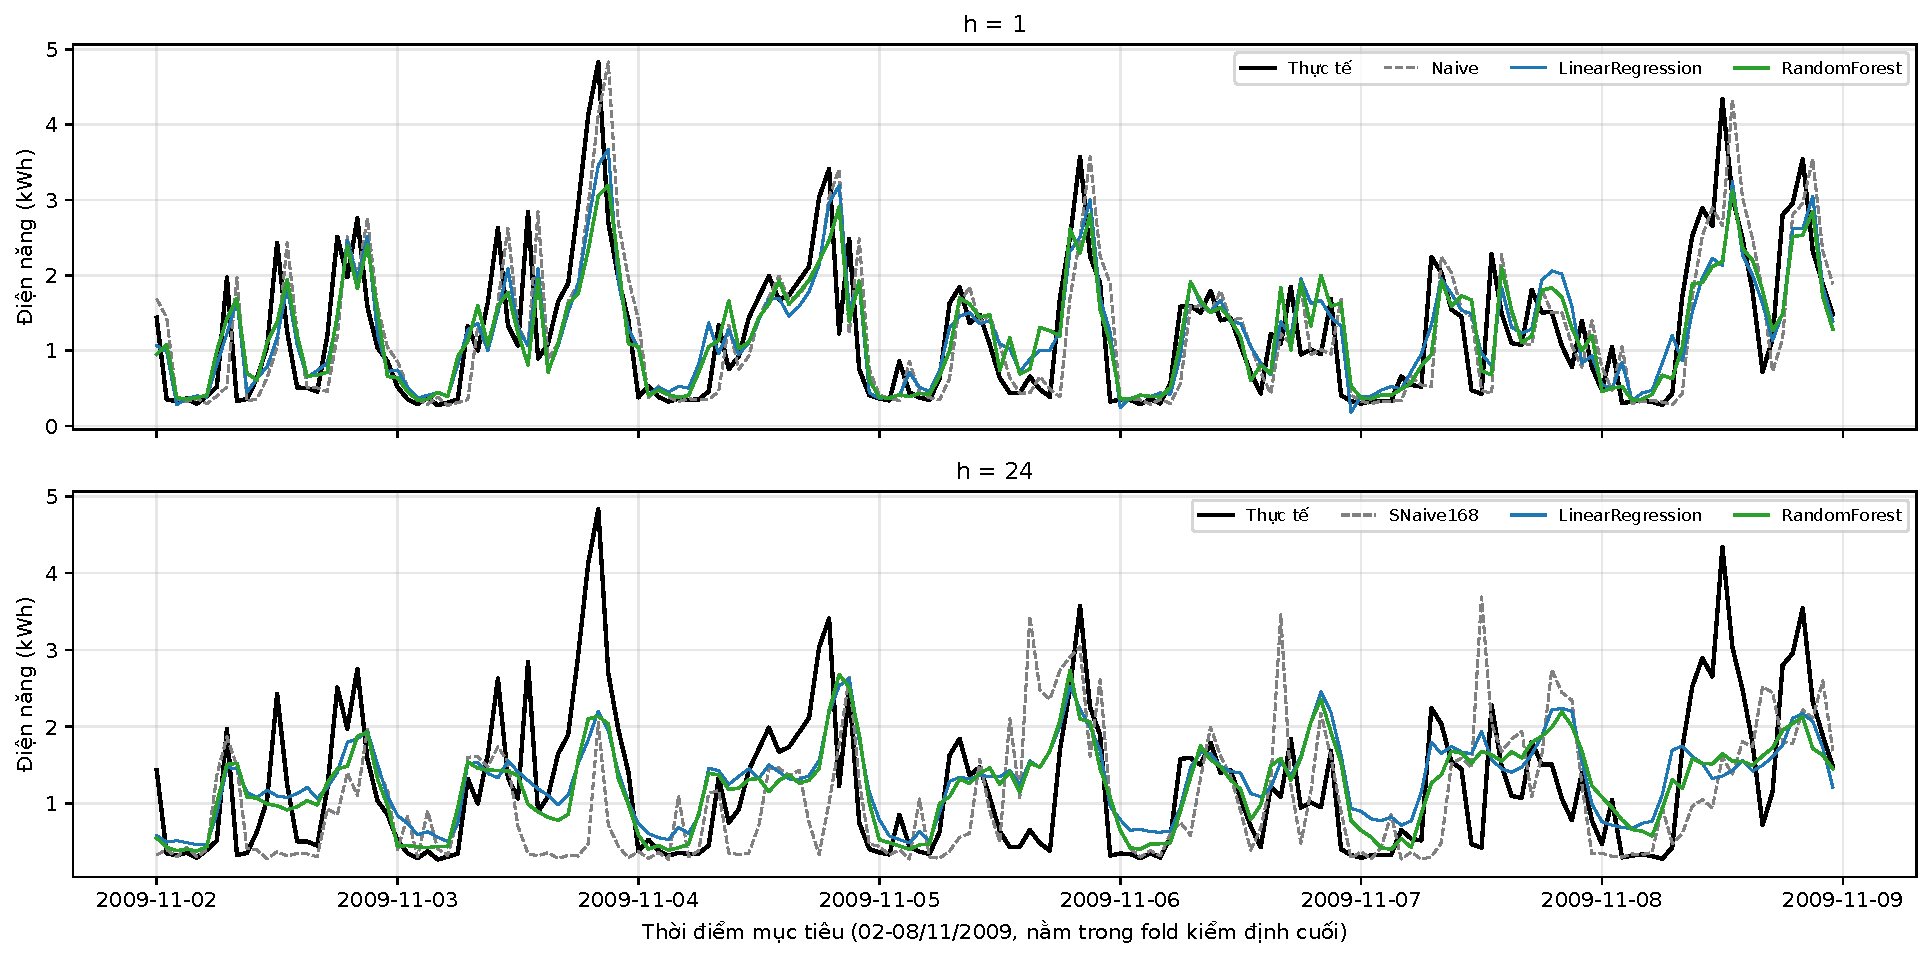
\includegraphics[width=\textwidth]{figures/tuan_vi_du.pdf}
    \caption{Dự báo và thực tế trong tuần 02--08/11/2009 (thuộc fold kiểm định cuối).}
    \label{fig:week}
\end{figure}

\paragraph{Ví dụ một tuần (Hình~\ref{fig:week}).} Với $h = 1$, các mô hình bám sát đường thực tế nhưng trễ khoảng một giờ ở các lần tăng đột ngột, và không đạt tới đỉnh 4,8 kWh tối 03/11 (Random Forest khoảng 3,2 kWh). Với $h = 24$, dự báo mượt hơn hẳn: mô hình tái hiện được nhịp tăng buổi tối hằng ngày nhưng gần như bỏ qua các đỉnh riêng lẻ, còn SNaive168 sao chép nguyên tuần trước nên có những đỉnh không xảy ra trong tuần này.

\section{Đặc trưng ảnh hưởng đến dự báo}
\label{sec:importance}

\begin{figure}[htbp]
    \centering
    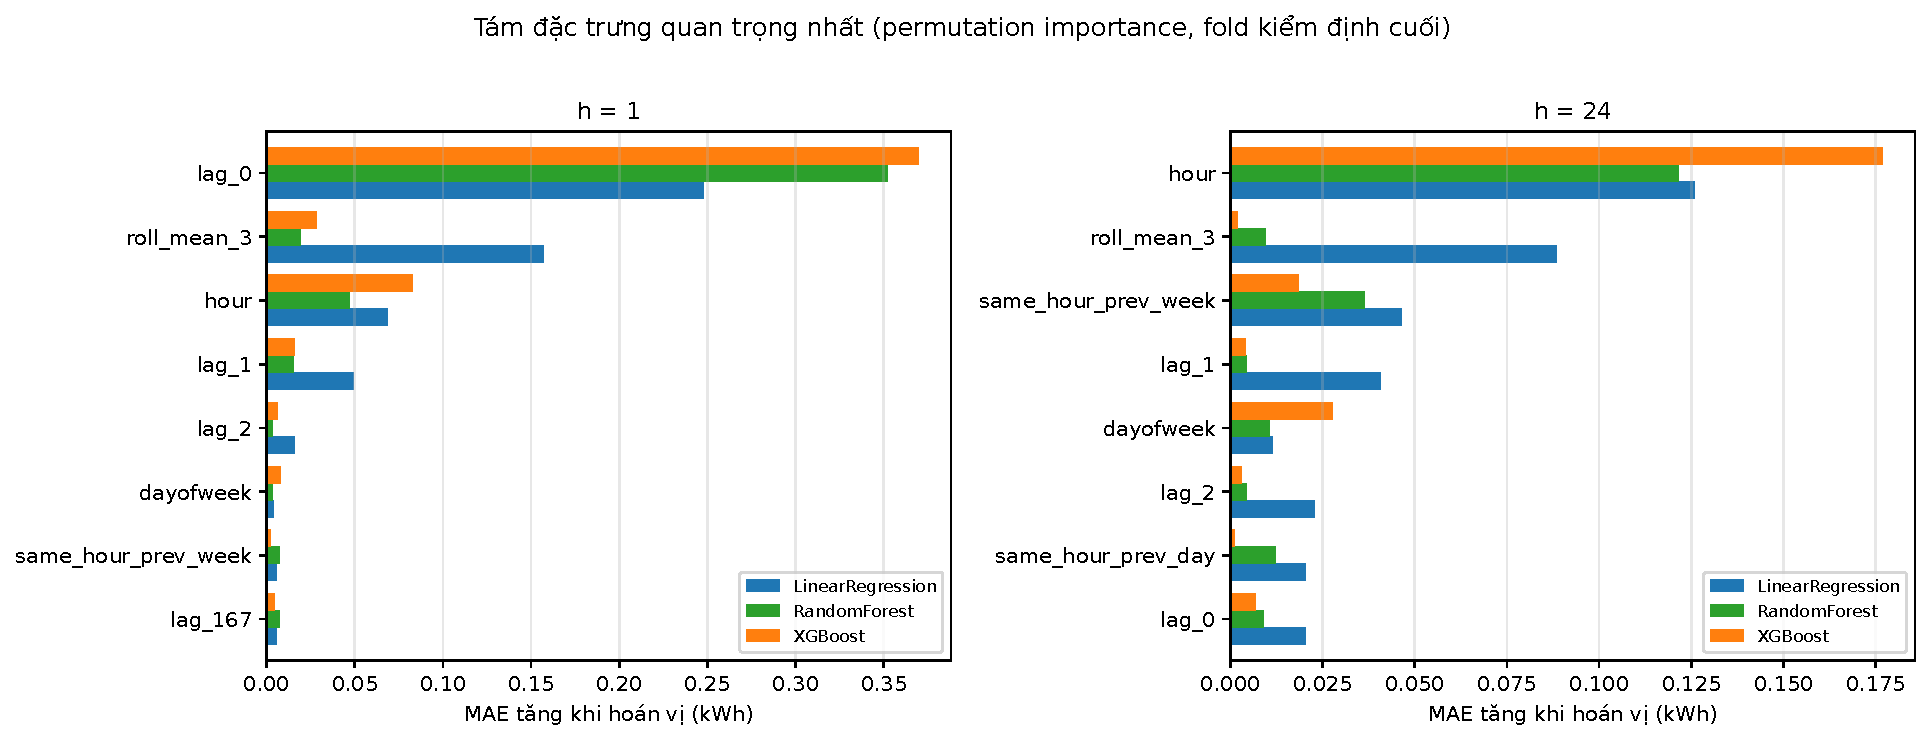
\includegraphics[width=\textwidth]{figures/tam_quan_trong.pdf}
    \caption{Tám đặc trưng quan trọng nhất theo permutation importance (MAE tăng khi hoán vị, phần kiểm định của fold cuối, 5 lần lặp).}
    \label{fig:importance}
\end{figure}

Hình~\ref{fig:importance} cho thấy cơ chế dự báo thay đổi theo tầm dự báo:
\begin{itemize}
    \item $h = 1$: thông tin về vài giờ vừa qua áp đảo. Với hai mô hình cây, hoán vị $y_t$ (điện năng giờ vừa qua) làm MAE tăng 0,35--0,37 kWh; Linear Regression chia tầm quan trọng này giữa $y_t$ (0,25) và trung bình 3 giờ gần nhất (0,16), vì trung bình này chứa chính $y_t$. Tiếp theo là giờ trong ngày (0,05--0,08).
    \item $h = 24$: giờ trong ngày trở thành quan trọng nhất (0,12--0,18 kWh), tiếp theo là giá trị cùng giờ tuần trước $y_{t+h-168}$ (0,02--0,05) và ngày trong tuần. Mô hình chủ yếu học hồ sơ tiêu thụ theo giờ và thứ, cộng với giá trị cùng giờ tuần trước.
\end{itemize}
Các đặc trưng tương quan với nhau chia sẻ tầm quan trọng; ví dụ ở $h = 24$, $y_t$ và giá trị cùng giờ ngày trước $y_{t+h-24}$ là cùng một giá trị. Kết quả này khớp với nhận xét ở Mục~\ref{sec:correlation}: tự tương quan bậc 1 cao quyết định dự báo ngắn hạn, còn chu kỳ ngày và tuần quyết định dự báo xa hơn.

\section{Thảo luận}
\label{sec:discussion}

\paragraph{Vì sao mô hình cây tốt hơn Linear Regression.} Điện năng phụ thuộc vào tương tác giữa giờ, thứ, tháng và mức tiêu thụ gần đây (ví dụ cùng là 20 giờ nhưng mùa đông và mùa hè khác nhau). Linear Regression chỉ cộng các tác động riêng lẻ nên chưa khớp; mô hình cây tự chia dữ liệu theo các tổ hợp này. Lợi thế của mô hình cây rõ nhất ở đỉnh buổi sáng và buổi tối, nơi tương tác giữa giờ và mức tiêu thụ trước đó mạnh nhất.

\paragraph{Vì sao lợi thế so với mô hình cơ sở gần như không đổi theo $h$.} Mức giảm MAE so với mô hình cơ sở tốt nhất là 17--20\% với Random Forest ở mọi $h$. Ở $h = 1$, mô hình cải thiện so với Naive nhờ biết giờ trong ngày; ở $h \ge 6$, mô hình cải thiện so với SNaive168 nhờ kết hợp nhiều chu kỳ thay vì sao chép một tuần duy nhất.

\paragraph{Hạn chế ở giai đoạn này.} (i) Siêu tham số chưa được tối ưu và mô hình cây có dấu hiệu quá khớp chưa được kiểm chứng đầy đủ. (ii) Mô hình dự báo thấp có hệ thống các giờ đỉnh. (iii) Bộ đặc trưng chưa có thông tin ngày lễ và giá trị trễ của các nhóm công tơ phụ. (iv) Kết quả mới là kiểm định chéo trên tập huấn luyện; tập kiểm tra năm 2010 sẽ chỉ được dùng một lần cho mô hình cuối ở giai đoạn tối ưu hóa, để ước lượng sai số trên dữ liệu mới không bị ảnh hưởng bởi các lựa chọn của nhóm.
